\documentclass[]{article}
\usepackage{hyperref}
\usepackage{multicol}
\usepackage{graphicx}
\usepackage{xcolor}
\usepackage{listings}
\usepackage{xparse}
\usepackage{float}
\usepackage{caption}
\usepackage{multicol}
\setlength{\columnsep}{0.7cm}
\usepackage[backend=bibtex]{biblatex}
\usepackage[a4paper, total={6in, 8in}]{geometry}
%opening
\title{ \textbf{Analysis of dopamine lateralization function in relation to Parkinson's symptoms}}
\author{Benedetta Corso, Letizia Rossato, Dalila Dattoli}
\date{}
\addbibresource{bibliog.bib}
\providecommand{\keywords}[1]
{
	\small	
	\textbf{\textit{Keywords--}} #1
}
\NewDocumentCommand{\codeword}{v}{%
	\texttt{\textcolor{blue}{#1}}%
}

\lstset{language=C,keywordstyle={\bfseries \color{blue}}}

\newenvironment{Figure}
{\par\medskip\noindent\minipage{\linewidth}}
{\endminipage\par\medskip}


\begin{document}

\maketitle

\begin{abstract}
This study, which focuses on Parkinson's disease, aims to investigate the significance of right-left lateralization on dopamine values using DAT-SPECT (Dopamine Transporter Single Photon Emission Computed Tomography) imaging data and their correlation with clinical symptoms in Parkinson’s disease patient (PD) and healthy controls (HC). DAT-SPECT is an imaging technique primarily used to visualize and measure the density of dopamine transporters in the brain. This technique is particularly useful in the diagnosis and evaluation of neurodegenerative diseases, such as Parkinson's disease and other forms of parkinsonism. The dataset, from PPMI, used to perform the analysis, consists of variables relating to demographic data, DAT-SPECT scores and MDS-UPDRS test, which is a combination of clinical, neurological, and imaging tests, since there is no specific test for the diagnosis of Parkinson’s disease. In order to investigate whether the lateralization is related to symptoms, a linear regression was used. This analysis verified that the lateralization present only in PD patients is highly related to symptoms.
\newline

\end{abstract}

\keywords{Parkinson's disease, dopamine lateralization, DAT-SPECT, MDS-UPRDS, SBR, motor symptoms, linear regression}


\vspace{5pt}
\hrule
\vspace{6pt}

\begin{multicols}{2}
\section{Introduction}
Parkinson's disease is a chronic neurodegenerative disorder of the central nervous system primarily affecting motor control. It is characterized by the progressive loss of nerve cells in the brain region called the substantia nigra, which is responsible for producing a neurotransmitter called dopamine. Dopamine deficiency leads to motor symptoms such as tremors, muscle rigidity, bradykinesia (slowness of movement), and postural instability. In addition to motor symptoms, Parkinson's disease can cause a wide range of non-motor symptoms including sleep problems, depression, anxiety, fatigue, and cognitive difficulties. While the exact cause of Parkinson's disease is not fully understood, it is believed to result from a combination of genetic and environmental factors \cite{beitz_parkinsons_2014}. Currently, there is no cure for Parkinson's disease, but there are treatments available to manage symptoms and improve the patients’ quality of life.  However, studies conducted in recent years \cite{shigekiyo_laterality_2020} have shown that the lateralization of brain dopamine in Parkinson's disease (PD) is a significant and distinctive aspect of the pathology. In particular, during its development, the degeneration of dopaminergic neurons in the substantia nigra is not uniform. Generally, one side of the brain is more affected than the other, leading to marked asymmetry. This marked asymmetry is visible especially in motor symptoms, such as more pronounced tremors on one side of the body and greater use of one hand over the other \cite{riederer_lateralisation_2018}. 
\newline
In previous studies, the connection between dopamine lateralization and symptoms has already been examined. For example, in a study conducted by Pirker et al. \cite{pirker_correlation_2003}, it resulted that the motor symptoms on the less affected side were more correlated to striatal DAT binding.
\newline
Therefore, the aim of this study is to further investigate this idea, analyzing a dataset containing information about patients' motor and cognitive symptoms and also their lateralization data obtained from DAT-SPECT scans. The dopamine degeneration is explored in three different Regions of Interests (ROIs) in the brain, divided in right and left: Caudate, Putamen and Putamen Anterior. This analysis aims to investigate whether there are some relevant covariates from HC associated to dopamine function lateralization, and furthermore, to investigate the relationship (if present) between the lateralization of dopamine function in these brain areas and the symptoms shown by Parkinson's patients. \cite{kagi_role_2010}
In addition, the group checked also if there was a difference in lateralization between HC and PD. 
\newline
Agreeing with what found in the paper by Pirker et al. \cite{pirker_correlation_2003}, the group expected to find a strong relation between the dopamine lateralization and the motor symptoms. The lateralization was expected to be significantly different between the two groups of HC and PD. Also the lateralization in different ROIs was expected to be related: a high lateralization in the Caudate was expected if both Putamen and Putamen Anterior were highly lateralized. Regarding the covariates, age was expected to be the variable most correlated to the dopamine function lateralization.

\section{Material and Methods}

\subsection{Dataset description}
The dataset used in this study was composed of 1556 subjects, of which 256 healthy controls and 1300 PD patients with different levels of symptoms' severity. Not all the variables given were interesting for the study. For example, all the data regarding the MRI acquisitions were discarded, because the analysis focused on the data from the DAT-SPECT scans.

The variables:
\begin{itemize}
	\item DATSCAN\_CAUDATE\_L
	\item DATSCAN\_CAUDATE\_R
	\item DATSCAN\_PUTAMEN\_L
	\item DATSCAN\_PUTAMEN\_R
	\item DATSCAN\_PUTAMEN\_ANT\_L
	\item DATSCAN\_PUTAMEN\_ANT\_R
\end{itemize}
contained the Striatal Binding Ratios (SBR) of the three ROIs (right and left sides), whether the scan was completed and its quality based on visual interpretation, as well as information regarding the date of the scan and the injection. 
\newline
The dataset included a part of demographics data, like age, ethnicity, gender, family members affected by PD, height, weight and dominant hand.
A total of 967 and 589 patients were males and females, respectively. The average age in the baseline was 62.69 ± 10.11 years (range [29.3–86.5]). 

There was then the data regarding the neuropsychological assessments of the patients using the Movement Disorder Society (MDS)-sponsored revision of the Unified Parkinson's Disease Rating Scale (MDS-UPDRS). The test is divided in 4 parts, concerning different classes of motor and cognitive symptoms, as specified in the PPMI Program Protocols \cite{marek_parkinsons_2018}. Each answer could range from 0 (normal) to 4 (severe), and for each part there was a summing-up variable, that contained the sum of all the scores of that section. These variables were called NP1PTOT, NP1RTOT, NP2TOT, NP3TOT, NP4TOT. Some motor symptoms in the third part, were divided in right and left, for example, the severity of tremor of the right or left upper limb. This was useful to investigate the different relation with the dopamine function lateralization.
\newline

\subsection{Cleaning e preprocessing}

The first step of the study was dividing the dataset in Parkinson's patients (PD, SWEDD (Scans without evidence of dopaminergic deficit), Prodromal (before the onset of classical Parkinson's symptoms)) and healthy controls (HC).

In the preprocessing of the data, the patterns of missing values were analyzed, to determine the best course of action, through the VIM package in R. \cite{missing_templ}

In the HC, as shown in Figure \ref{fig:miss_patt_hc}, GENETICS and FAMILIARITY are mostly empty fields, due to the nature of these variables: for healthy subjects, the chance of having relatives with a PD diagnosis and of having genetics history related to PD are low. On the opposite, for PD patients (Figure \ref{fig:miss_patt_pd}), GENETICS is empty at the 24.5\%, while FAMILIARITY has the 47.7\% of NaNs. The reason for this missingness, is probably that patients didn't know if their relatives had history of Parkinson's, or they didn't take the genetics test. 

In the complete dataset, NP4TOT is missing at the 73.9\%; nearly all the HC didn't take the fourth part of the test, and also the participation of the PD was really low. This suggests that the fourth part of the test was taken by a few subjects. For this reason, the NP4 variables were not taken into account in the statistical analysis.

For all the test-related variables (NP1PTOT, NP1RTOT, NP2TOT, NP3TOT), both in HC and PD, if a subject is missing a value for one test, also the other tests' results are missing. The pattern of missing data is considered to be MAR (Missingness At Random). For the statistical analysis, all the subjects that were missing at least one test result weren't considered.  

For ETHNICITY, SEX, and HAND (dominant hand of the subject), there aren't missing valules in the whole dataset. In the ENROLL\_AGE variable, the missing values were calculated using the DAT-SCAN date and the birth date of the subject.

Regarding HEIGHT and WEIGHT, the pattern of missing data is MAR, with a total of 33.3\% of NaNs. 

The variable PRIM\_DIAG described the primary diagnosis; the group found some subjects with the value of 97, that wasn't explained by the data dictionary, therefore it was removed both from the HC and from the PD. 

In Figures \ref{fig:miss_val_hc} and \ref{fig:miss_val_pd}, all the combinations of missing values of the dataset have been represented, using the VIM package in R.
\end{multicols}

\begin{figure}[h]
	\centering
	\parbox{2.8in}{
		\centering
		\includegraphics[width=2.5in]{../missing_patterns_hc}
		\caption{Pattern of missing values in HC}
		\label{fig:miss_patt_hc}}
	\begin{minipage}{2.8in}
		\centering
		\includegraphics[width=2.5in]{../missing_patterns_pd}
		\caption{Pattern of missing values in PD}
		\label{fig:miss_patt_pd}
	\end{minipage}
\end{figure}

\begin{figure}[h]
	\centering
	\parbox{2.8in}{
		\centering
		\includegraphics[width=2.5in]{../missing_values_hc}
		\caption{Missing values in HC}
		\label{fig:miss_val_hc}}
	\begin{minipage}{2.8in}
		\centering
		\includegraphics[width=2.5in]{../missing_values_pd}
		\caption{Missing values in PD}
		\label{fig:miss_val_pd}
	\end{minipage}
\end{figure}

\begin{multicols}{2}

Another reason of exclusion from the analysis, was having an incomplete DAT-SCAN, a scan with poor quality, or, just for HC, a MoCA (Montreal Cognitive Assessment - stored in the variable MCATOT), score lower than 26. This test assesses the cognitive impairment, and, under 26, the subjects couldn't be considered healthy. 

The preprocessing step ended with the removal of some outliers from ENROLL\_AGE, HTCM and WGTKG. The ouliers of weight were 14 in PD patients and 42 in HC; for height just 2 PD were considered outliers, while, looking at age, 4 PD and 8 HC were removed as outliers.

Concerning the demographics data, the two datasets were compared, to see if they had the same distributions. Through the Lilliefors test (MATLAB function \codeword{lillietest}), the gaussianity of age, height and weight was checked. For the gaussian variables, the Anova test (MATLAB function \codeword{anova1}) was used to compare the population means, while for the not gaussian ones, the Wilcoxon test was applied (MATLAB function \codeword{ranksum}). The average values of age, height and weight were found identical for the two groups. The proportion of male and female was comparable: in the whole dataset, the proportion of females was 37,85\%, while in PD was 38,5\% and in HC 34,37\%. 

The distribution of ETHNICITY was also found similar between the two groups, while FAMILIARITY and HAND were significant different in the two populations when analyzed through a Wilcoxon test. The differences in FAMILIARITY can be explained by the connection between PD patients and the genetic components in the disease: for a PD patient, it's more likely to have some relatives affected by PD, than for an healthy subject. The difference in HAND is due to the composition of the dataset; therefore, for this reason, and because there weren't enough left-handed subjects, this variable wasn't used in the analysis.

\subsection{Feature extraction}

In order to perform the statistical analysis to answer the study questions, the relevant features were extracted.
The analysis was based on the DAT-SPECT data, for the three ROIs, the demographic data and the symptoms tests results.

\subsection{Lateralization coefficients}

From the lateralization data, the group used a DAT binding asymmetry coefficient found in a study conducted by Kaasinen et al. \cite{kaasinen_ipsilateral_2016}: 
\begin{equation}
	\frac{(right_{SBR} - left_{SBR})}{(right_{SBR} + left_{SBR})}
\end{equation}
The lateralization was considered relevant when the asymmetry coefficient was higher than 20\%.
This threshold level was adopted from a previous study \cite{fiorenzato_asymmetric_2021}. 
This coefficient was used just to count the subjects with a relevant lateralization, while in the statistical analysis, all the subjects were considered.

\subsection{Covariates analysis}

In this section, the group investigated whether there was any relevant covariate from HC associated to dopamine function lateralization.
Analyzing HC, the possible covariates were sex, dominant hand, ethnicity, age, height, weight.

Regarding the discrete variables, it was possible to analyze only SEX, because the others didn't divide the subjects in groups with a comparable number of data.

For the analysis of the covariate SEX, the lateralization coefficients were, for each region, divided in males and females. Through a Lilliefors test, both groups were found not gaussian. Therefore, they were compared with a Wilcoxon test, finding that only for Putamen Anterior, males and females had different medians of lateralization coefficients.
Consequently, SEX was considered as a covariate for Putamen Anterior lateralization data, and the statistical analysis on PD patients was performed both on the whole group and on the two sub-groups of males and females for this brain region.

Through the Pearson pairwise correlation, the group analyzed the correlation coefficients of the continue variables, such as ENROLL\_AGE, WGTKG (weight - kg), HGTCM (height - cm), with the lateralization coefficients (Figures \ref{fig:cov_mat_hc}). For the statistical analysis, were kept only the significant ones, with p-value $<$ 0.05, and correlation coefficient higher than 0.5. This threshold was chosen in order to have at least a moderate correlation (0.4-0.59). 

\begin{Figure}
	\centering
	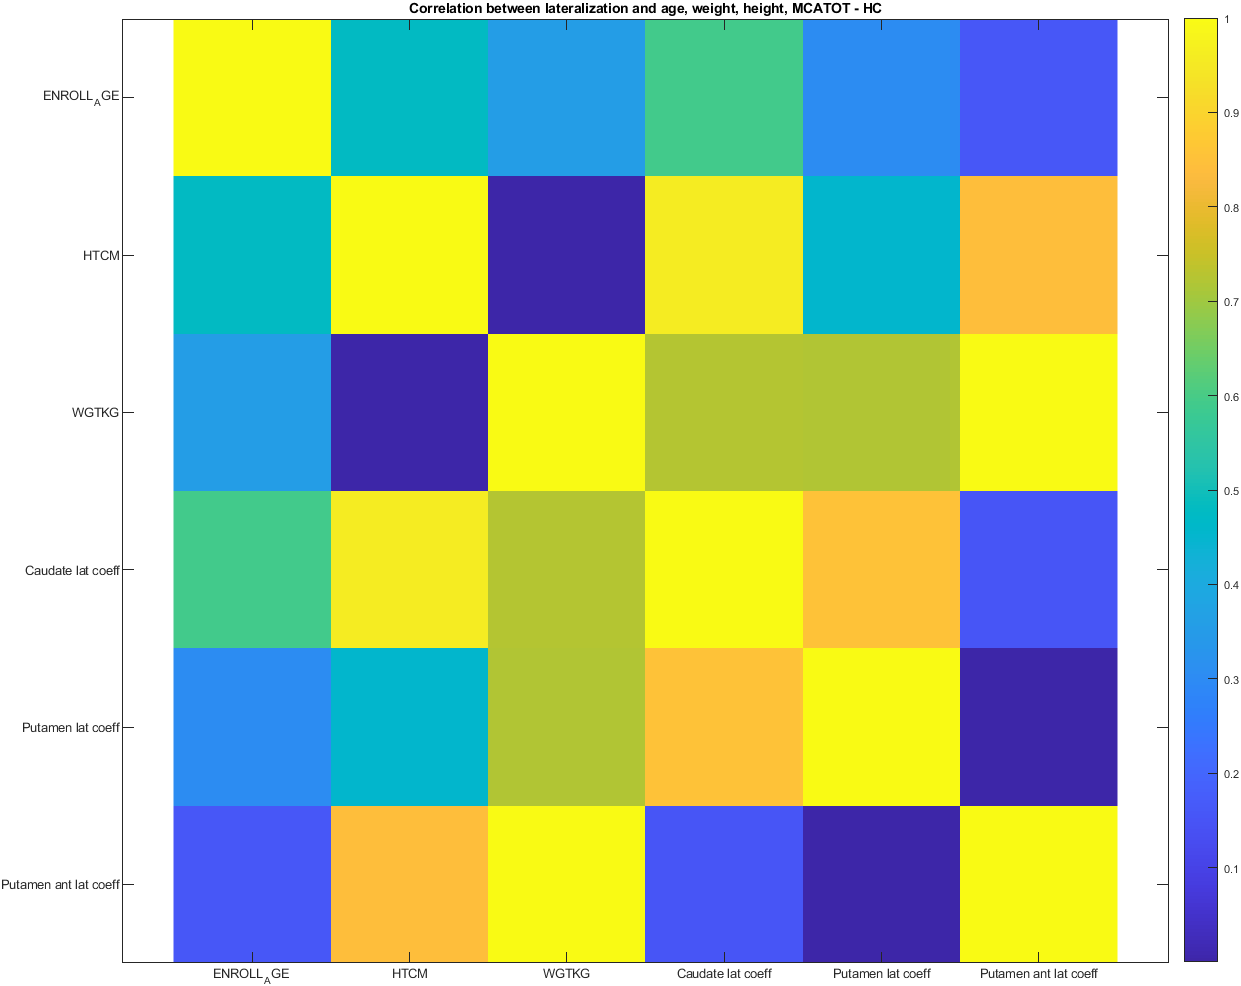
\includegraphics[width=2in]{../covariates_mat_hc}
	\captionof{figure}{Correlation matrix between covariates and lateralization coefficient - HC}
	\label{fig:cov_mat_hc}

\end{Figure}
 
In the correlation matrix of the HC in Figure \ref{fig:cov_mat_hc}, it's shown that ENROLL\_AGE has a moderate correlation only with the lateralization coefficient in the Caudate region, while it has a weak correlation with the other two ROIs. HTCM is strongly correlated with Caudate's lateralization coefficient, moderately with Putamen and has a very strong correlation with Putamen Anterior. Similarly, also WGTKG has a very strong correlation with Putamen Anterior, and a strong one with Caudate and Putamen lateralization coefficients.

\subsection{Statistical methods}

The group used the Pearson correlation coefficient in the covariates analysis and in the symptoms analysis.

The Anova test was used in the pre-processing section in order to compare the distributions of HC and PD continuous variables (age, height, weight).
Also, the Wilcoxon test was used during the pre-processing step, but to compare the discrete variables distributions (sex, familiarity, ethnicity).

Then the group compared HC and PD populations in terms of lateralization, using a Wilcoxon test (Figure \ref{fig:anova_plot}). The Wilcoxon test was chosen because the normality assumption wasn't met, and so the T-test couldn't be used.
Therefore, the analysis investigated the presence of a difference between the lateralization in HC with the one in PD. To perform the analysis, the lateralization was taken in absolute value. The choice of using the absolute value came from the interest on the amount of lateralization, not its direction.

\subsubsection{Linear regression}

Using the covariates variables (found for HC through the correlation matrix) and the symptoms data, the group performed a linear fit with the lateralization coefficients of PD patients, to check the presence of a linear relation between them. To improve this fit, the covariates were chosen looking at the best value of the adjusted $R^2$ obtained from the comparison of all the fits with all the possible covariates combinations. 
This was implemented through the MATLAB function \codeword{fitlm} (the lateralization was not take in absolute value, in order to have a relation with its direction).
As parameter, the adjusted $R^2$ was used to get the true value of the fit.

\section{Results}

A seen in the pre-processing step, the 2 groups of HC and PD were similarly distributed, and therefore the following analysis could be performed.

The covariates extracted for each ROI are shown in Table \ref{tbl:cov_hc}.



\begin{center}
	\centering
	\tiny
	\begin{tabular}{|c|c|c|}
		\hline
		\textbf{ROIs}             & \textbf{Covariates} & \textbf{Correlation coefficient} \\ \hline
		\textbf{Caudate}          & ENROLL\_AGE         & 0.593                            \\ \hline
		\textbf{}                 & HTCM                & 0.958                            \\ \hline
		\textbf{}                 & WGTKG               & 0.723                            \\ \hline
		\textbf{Putamen}          & WGTKG               & 0.722                            \\ \hline
		\textbf{Putamen Anterior} & HTCM                & 0.840                            \\ \hline
		\textbf{}                 & WGTKG               & 0.997                            \\ \hline
	\end{tabular}
	\captionof{table}{Covariates correlation coefficients - HC}
	\label{tbl:cov_hc}
\end{center}


\subsection{Comparison between HC and PD lateralizations}

The boxplot comparing the lateralization coefficients of PD and HC is shown in Figure \ref{fig:anova_plot}.
As hypothesized at the start of the study, the analysis confirmed that there was a significant difference (p-value $<$ 0.01) in the lateralization of HC and PD in all the ROIs.
Using the lateralization coefficient threshold, the group identified, for the Caudate, 28 PD patients with a right lateralization and 29 with a left lateralization. For the Putamen, 203 PD had a right lateralization, 2 HC and 150 PD with a left lateralization. For the Putamen Anterior, 113 PD patients were found lateralized on the right side, while 64 on the left. The remaining subjects were not lateralized.

\begin{Figure}
	\centering
	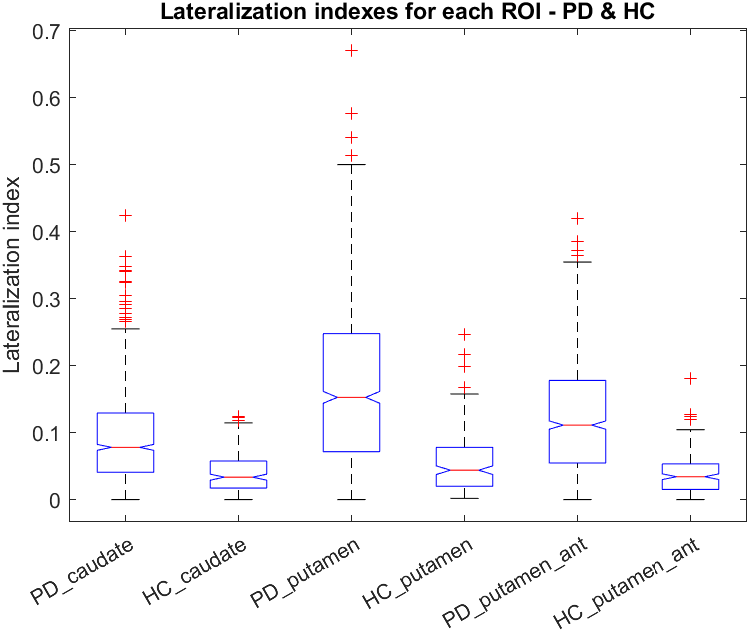
\includegraphics[width=3in]{../anova_plot_lat_hc_pd}
	\captionof{figure}{Boxplot comparing lateralization coefficients in PD and HC}
	\label{fig:anova_plot}
\end{Figure}

\subsection{Symptoms correlation matrix}

To answer the second research question, which was to investigate the relationship between dopamine lateralization function and symptoms, the group extracted the significant symptoms from a correlation matrix (Figure \ref{fig:corr_symp_pd}) obtained with the Pearson correlation as done for the covariates, with a threshold of 0.5 for the correlation coefficients. 


\begin{Figure}
	\centering
	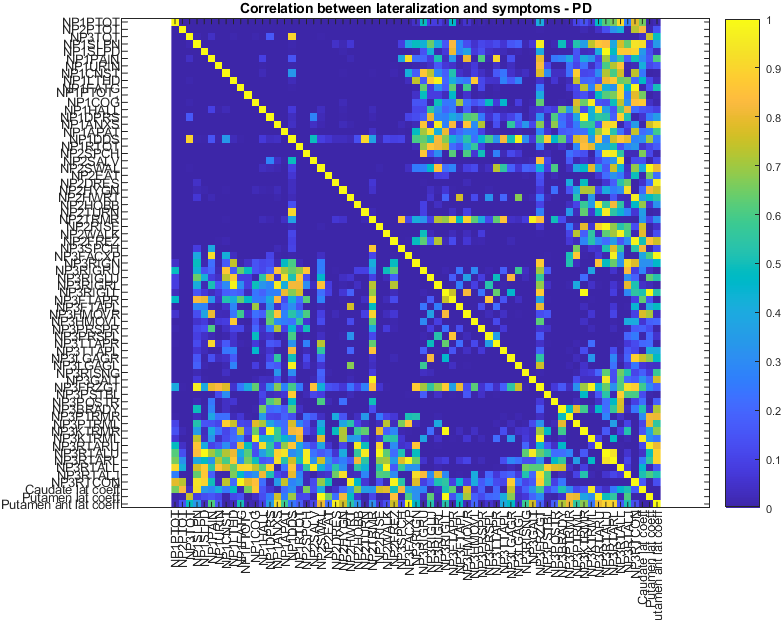
\includegraphics[width=3in]{../corr_mat_symptoms_pd}
	\captionof{figure}{Correlation matrix between Lateralization coefficients and symptoms - PD}
	\label{fig:corr_symp_pd}
\end{Figure} 


\subsection{Linear fit with covariates and symptoms}

These symptoms were used, together with the covariates found from HC, to perform a linear fit with the lateralization coefficients in PD, in order to find the relationship between dopamine lateralization function and symptoms. The graphs of the fit are shown in Figure \ref{fig:lin_fit_pd}. The graphs contain on the x-axis the covariates and the symptoms, while on the y-axis the lateralization coefficients. Each figure shows the fit for the three different ROIs, Caudate, Putamen and Putamen Anterior. 

To improve the fit, the group chose the best combination of covariates among the ones found before, using as selection criteria the adjusted $R^2$ value of the models tried with all the possible combinations. The selected covariates are listed in Table \ref{tbl:R_squared_fit_pd}. 
In this way, the sensitivity of the model to the various covariates was studied.

The numerical results of these linear fits are shown in the Table \ref{tbl:R_squared_fit_pd}, where $R^2$ (adjusted) was chosen because of the large amount of variables, in order to retrieve a more accurate value (see \cite{analysis_of_covariance_and_alternatives}). The p-values were all below 0.05 and so were significant.

\begin{Figure}
	\centering
	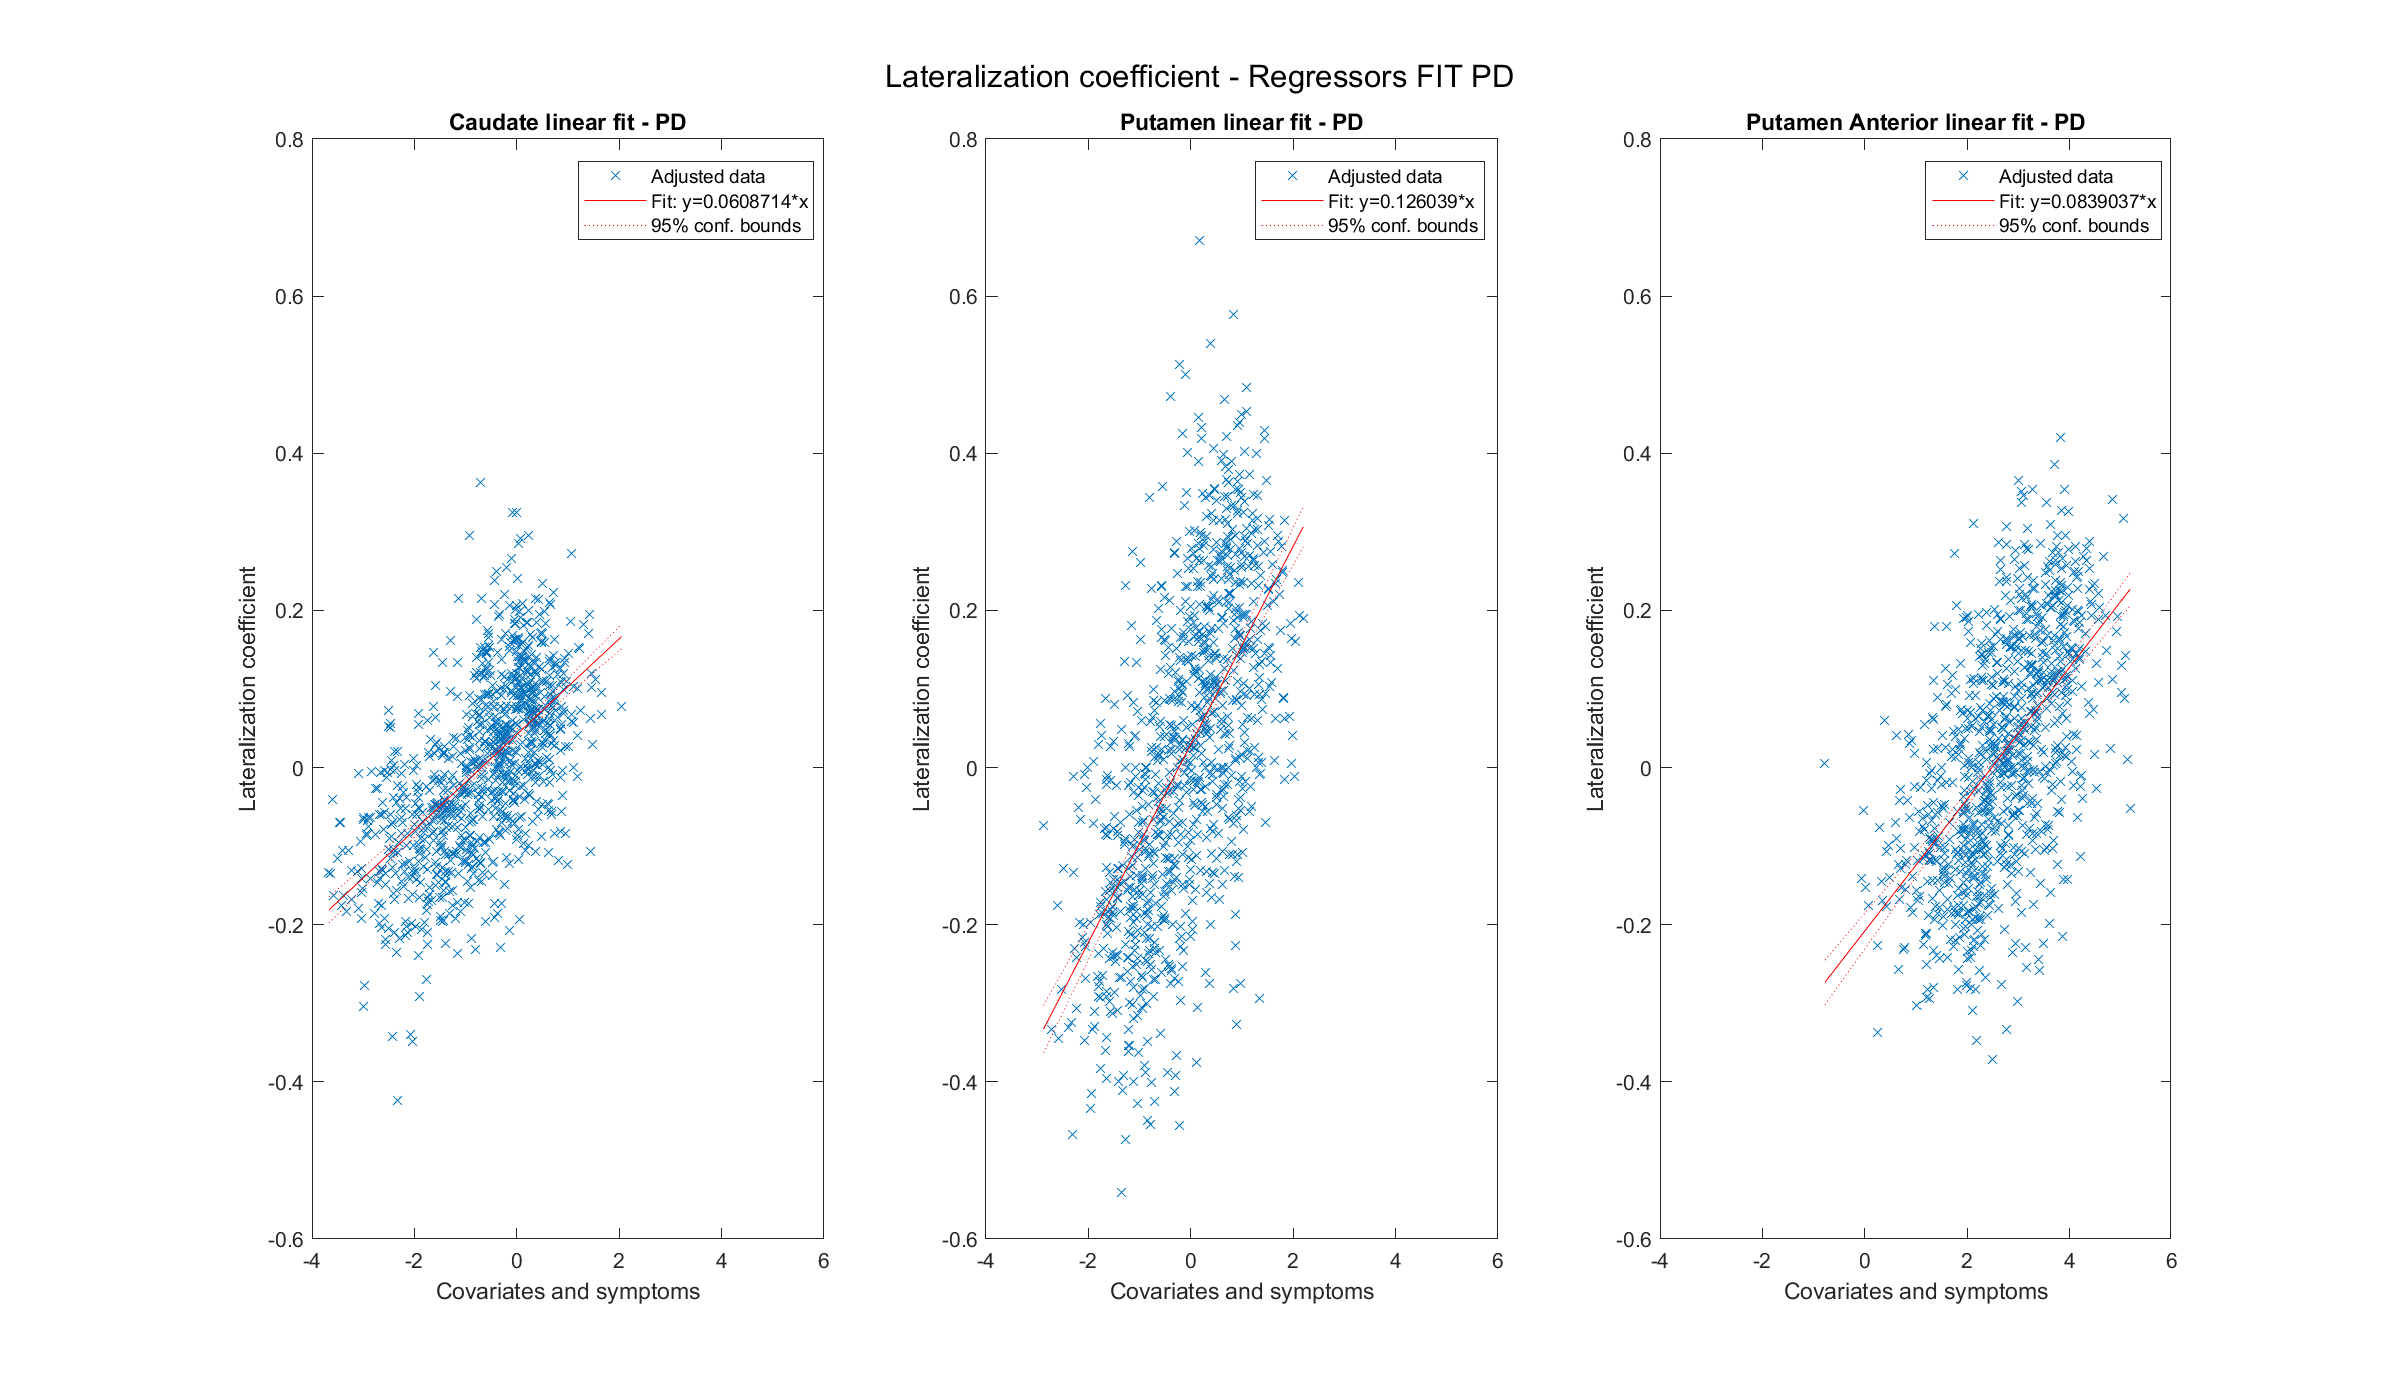
\includegraphics[width=3in]{../fit_covariates_pd}
	\captionof{figure}{Linear fit - PD}
	\label{fig:lin_fit_pd}
\end{Figure} 


\begin{center}
	\centering
	\tiny
	\begin{tabular}{|c|c|l|}
		\hline
		\textbf{ROIs}             & \textbf{Adjusted $R^2$} & \textbf{Covariates} \\ \hline
		\textbf{Caudate}          & 0.3343                  & HTCM                \\ \hline
		\textbf{Putamen}          & 0.3673                  & None                \\ \hline
		\textbf{Putamen Anterior} & 0.3014                  & HTCM, WGTKG         \\ \hline
	\end{tabular}
	\captionof{table}{Adjusted $R^2$ values of the linear fit between lateralization and symptoms}
	\label{tbl:R_squared_fit_pd}
\end{center}



\subsection{Linear fit with covariates and symptoms - gender division}

The linear fit on the Putamen Anterior was repeated for two sub-groups of patients - males and females, always selecting the best covariates from all the possible combinations. The fit are shown in Figure \ref{fig:lin_fit_male_female}, the p-values were all $<$ 0.05, while the adjusted $R^2$ values are shown in Table \ref{tbl:lin_fit_put_ant} for both males and females.


\begin{Figure}
	\centering
	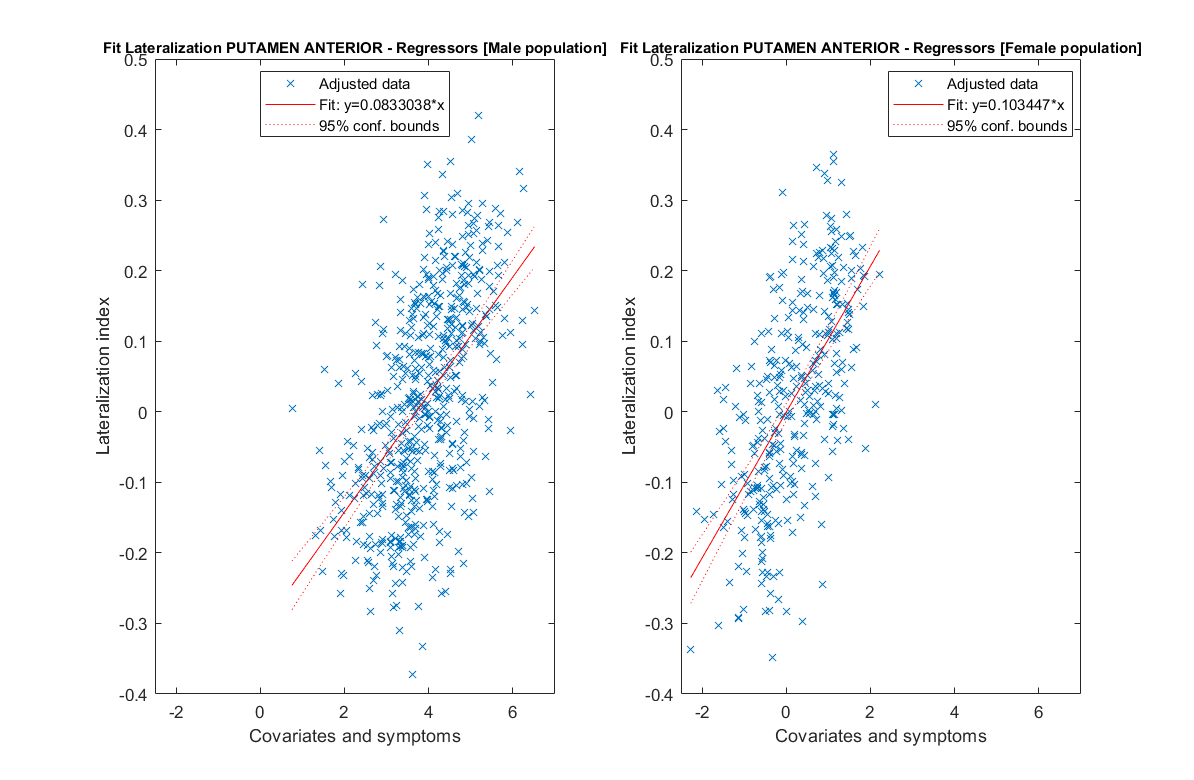
\includegraphics[width=3in]{../fit_covariates_male_female}
	\captionof{figure}{Linear fit for males and females - PD}
	\label{fig:lin_fit_male_female}
\end{Figure} 

\begin{center}
	\centering
	\tiny
	\begin{tabular}{|c|c|l|}
		\hline
		\textbf{Putamen Anterior} & \textbf{Adjusted $R^2$} & \textbf{Covariates} \\ \hline
		\textbf{Males}            & 0.2721                  & HTCM, WGTKG         \\ \hline
		\textbf{Females}          & 0.3523                  & WGTKG               \\ \hline
	\end{tabular}
	\captionof{table}{Adjusted $R^2$ for the linear fit of Putamen Anterior for males and females}
	\label{tbl:lin_fit_put_ant}
\end{center}


\section{Discussion}

In the analysis of the dataset, the extraction of the lateralization coefficient, based on \cite{kaasinen_ipsilateral_2016}, allowed to verify the difference between HC and PD. With the threshold at 20\%, the group verified that the strongly lateralized subjects were present only among PD patients, except for two outliers. 

The first aim of the study was to assess whether there were some relevant covariates associated to dopamine function lateralization. To do so, the analysis consisted in computing the correlation matrix between the lateralization data and the possible covariates in HC. Only the variables with at least a moderate correlation were selected as covariates. Analyzing these results (Table \ref{tbl:cov_hc}), the group concluded that weight was the only covariate associated to all the three regions of interest; therefore it's probable that a patient with a high body weight, and consequent high probability of health complications, will show a stronger lateralization of dopamine function. With respect to age, the analysis showed that the initial hypothesis wasn't verified for every ROI; in fact, age had a moderate correlation only with Caudate, while it was initially hypothesized to have a strong correlation with all the brain areas.

The group understood that there wasn't any significant lateralization in the HC, and therefore the linear fit wasn't appropriate to describe its relation with the symptoms.

The second research question concerned the relationship between the lateralization of dopamine function in the ROIs and the symptoms of PD patients.
As shown in Figure \ref{fig:lin_fit_pd} and in Table \ref{tbl:R_squared_fit_pd}, for PD patients, the values of $R^2$ and p-value are highly significant, showing that the lateralization is related to the symptoms, as hypothesized. The conclusion is that with a higher lateralization, there will be stronger symptoms.

Subsequently, the group performed the same analysis dividing the subjects between males and females for the Putamen Anterior lateralization data.

As shown in Table \ref{tbl:lin_fit_put_ant}, considering the covariate of gender, the linear fit of the lateralization data gets worse for males and improves for females.
Considering the whole population, the adjusted $R^2$ is in the middle of the values of the two groups because males and females compensate for each other. The difference between the values is not relevant; therefore it's not significant enough to generalize it.

\subsection{Limitations}

The dataset used in the study was not optimal for the study aim, as the amount of missing data penalized the analysis. A lot of subjects didn't take the fourth part of the symptoms assessment test, forcing the group to leave the collected data about NP4 outside the analysis. 
Another limitation of the dataset was its scarce variability in demographic data. In fact, as there weren't enough subjects with an ethnicity different from white, this variable couldn't be examined as covariate in the study. The same applied for the dominant hand variable. 
The analysis was centered on PD patients, including SWEDD and Prodromal subjects, but didn't investigate the possible influence of other diseases or conditions of the subjects at the moment of the study. Therefore, it can't be totally generalized without further investigation. 

\subsection{Future suggestions}

To further improve the study in case of future tries to analyze the dopamine lateralization in relation with symptoms, it would be necessary to choose a dataset with a larger variability, especially in demographic data (as ethnicity). It's not necessary to enlarge the dataset dimension, but an increase in subjects variability could improve the study generalizability.
It could also help to assure the presence of data for as many subjects as possible in all the symptoms assessment tests, in order to complete the analysis considering every possible symptom (motor and cognitive). 
Another important factor would be to assure the quality of the DAT-SPECT scans and of the consequent SBR extraction. 

Maybe with future studies, it will be possible to assess the nature of the relationship between lateralization and symptoms, eventually helping the creation of a new biomarker for PD diagnosis, since the loss of dopaminergic neurons is present even in the early stages of the disease before the onset of motor symptoms. \cite{booij_spect_2007}

Like in the study \cite{lorio_combination_2019} by Lorio et al., another strategy could be combining DAT-SPECT data with MRI data to have a more accurate biomarker and so a more accurate analysis.


\end{multicols}

\printbibliography
\end{document}
